\documentclass[11pt,a4paper]{article}
\ifdefined\pdfgentounicode
  \usepackage[utf8]{inputenc}
\fi
\usepackage[T1]{fontenc}
\usepackage[margin=2.25cm]{geometry}
\usepackage{amsmath,booktabs,catchfile,graphicx,tabularx,xcolor}
\usepackage[colorlinks=true,urlcolor=blue!55!black]{hyperref}
\ifdefined\pdfgentounicode
  \input{glyphtounicode}
  \pdfgentounicode=1
\fi
\CatchFileDef{\linhasValidacao}{tabela_validacao_cruzada.tex}{}
\CatchFileDef{\linhasTeste}{tabela_comparacao_teste.tex}{}

\definecolor{azulescuro}{HTML}{173A50}
\newcommand{\status}[1]{\texttt{PAY\_#1}}
\renewcommand{\thesection}{\Roman{section}}
\setlength{\parindent}{0pt}
\setlength{\parskip}{5pt}
\raggedbottom
\hypersetup{pdftitle={Tema 4 — Inadimplência de cartão de crédito},
  pdfsubject={Trabalho final de Mineração de Dados — UFU}}

\begin{document}
\noindent{\large\bfseries Universidade Federal de Uberlândia}\\
Ciência da Computação \enspace|\enspace Mineração de Dados \enspace|\enspace Elaine Ribeiro Faria

\vspace{6pt}
{\color{azulescuro}\par\Large\bfseries Tema 4: classificação de inadimplência\\ de cartão de crédito\par}
\smallskip
\begin{tabular}{@{}ll@{}}
\textbf{Integrante} & \textbf{Matrícula}\\
Matheus Medrado Ferreira & 12311BCC054\\
Christian Silva Rodrigues & 12311BCC025\\
Lucas Belchior & 12311BCC068\\
\end{tabular}
\par\smallskip
\textbf{Entrega no Microsoft Teams:} 24/11/2026, às 12h.

\section{Introdução e objetivos}
O trabalho compara quatro modelos que tentam prever se um cliente ficará
inadimplente no mês seguinte. Para isso, usamos dados que já estavam disponíveis,
como o limite do cartão, o valor das faturas e o histórico de pagamentos.

Testamos duas configurações de cada modelo. Além de comparar as métricas,
observamos os tipos de erro: deixar passar um inadimplente ou sinalizar
um cliente que não ficou inadimplente.

\section{Descrição da base de dados}
Usamos \href{https://archive.ics.uci.edu/dataset/350/default+of+credit+card+clients}{Default of Credit Card Clients (UCI 350)},
base histórica de Taiwan com registros de abril a setembro de 2005 e alvo
relativo ao mês seguinte. O Excel contém 30.000 registros e 25 colunas:
23 preditores, um identificador e o alvo. A tabela agrupa os campos mensais.

\begingroup\small
\begin{tabularx}{\linewidth}{@{}l l X@{}}
\toprule
\textbf{Coluna(s)} & \textbf{Tipo semântico} & \textbf{Significado}\\
\midrule
\texttt{ID} & Identificador & Identificador no arquivo; excluído dos modelos.\\
\texttt{LIMIT\_BAL} & Numérico & Limite de crédito concedido (NT\$).\\
\texttt{SEX} & Categórico & 1 = masculino; 2 = feminino.\\
\texttt{EDUCATION} & Categórico & 1 = pós-graduação; 2 = universidade; 3 = ensino médio; 4 = outros.\\
\texttt{MARRIAGE} & Categórico & 1 = casado; 2 = solteiro; 3 = outros.\\
\texttt{AGE} & Numérico discreto & Idade em anos.\\
\status{0}, \status{2} a \status{6} & Categórico & Status mensal: $-1$ = em dia; 1 a 8 = meses de atraso; 9 = nove meses ou mais. Ordem das colunas: setembro a abril.\\
\texttt{BILL\_AMT1} a \texttt{6} & Numérico & Valor mensal da fatura (NT\$), de setembro a abril.\\
\texttt{PAY\_AMT1} a \texttt{6} & Numérico & Valor pago por mês (NT\$), de setembro a abril.\\
\texttt{default payment} & Classe binária & \texttt{next month}: 0 = não houve inadimplência; 1 = houve inadimplência.\\
\bottomrule
\end{tabularx}
\endgroup

\newpage
\subsection*{Distribuição do alvo e qualidade dos dados}
No mês seguinte, 23.364 clientes (77,88\%) não ficaram inadimplentes
(classe 0) e 6.636 (22,12\%) ficaram inadimplentes (classe 1). A base
é desbalanceada, com cerca de três clientes da classe 0 para cada cliente
da classe 1. As figuras mostram essa diferença e as distribuições de idade e limite.

\begin{center}
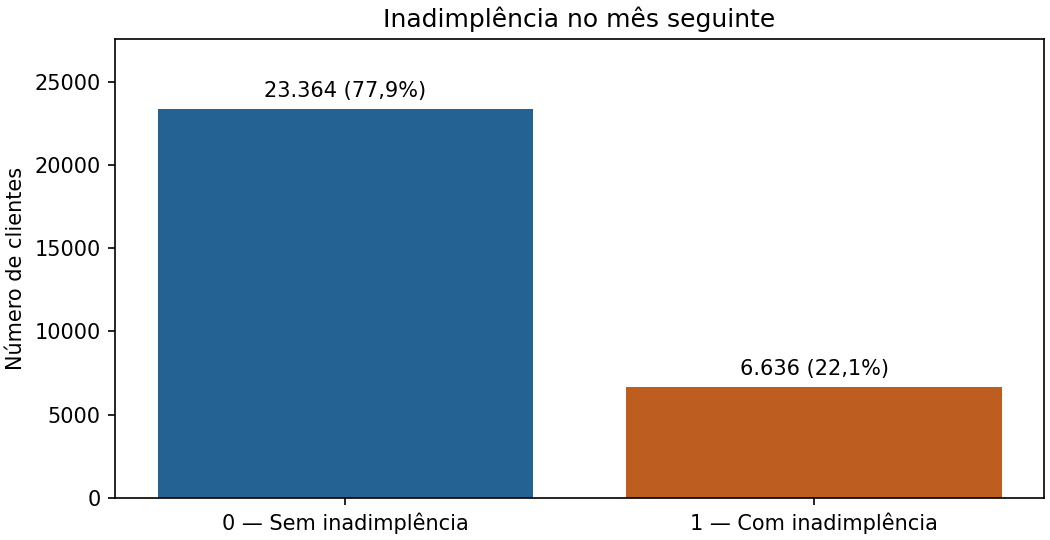
\includegraphics[width=.68\linewidth]{figures/eda_classes.png}\\[-2pt]
{\small\textbf{Figura 1.} Contagens por classe no conjunto completo.}

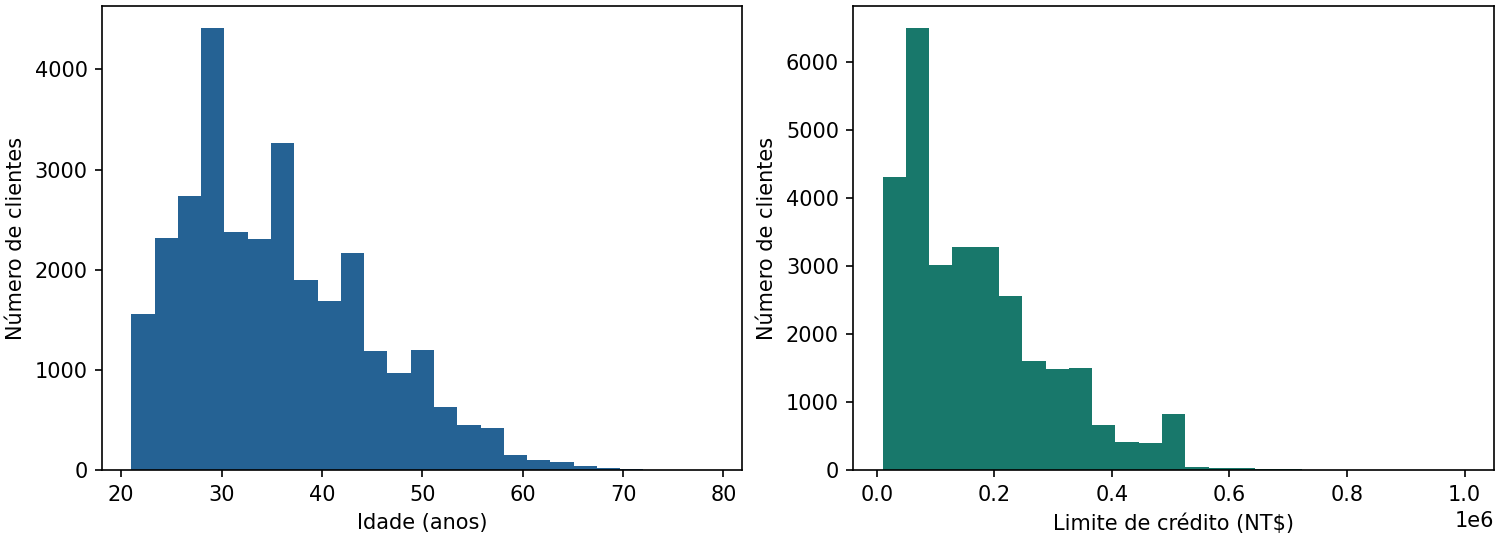
\includegraphics[width=.90\linewidth]{figures/eda_idade_limite.png}\\[-2pt]
{\small\textbf{Figura 2.} Distribuições de idade e limite de crédito.}
\end{center}

\begin{itemize}
  \item Não há células vazias, IDs repetidos nem linhas completas duplicadas.
  Sem ID, mas mantendo o alvo, há 35 linhas iguais além da primeira
  ocorrência. Considerando só os preditores, há 56 repetições além da primeira
  ocorrência: 108 registros distribuídos em 52 grupos de perfis idênticos.
  Desses grupos, 21 têm alvos diferentes.
  \item A planilha contém códigos não descritos na ficha da UCI:
  \texttt{EDUCATION} 0 (14 registros), 5 (280) e 6 (51);
  \texttt{MARRIAGE} 0 (54); e status de pagamento $-2$ e 0 nos seis meses.
  Conforme o mês, o código $-2$ aparece de 2.759 a 4.895 vezes e o 0 de
  14.737 a 16.947 vezes. Eles não foram tratados como ausências.
  \item Há valores negativos em todas as colunas de fatura, de 590 a 688
  por coluna. Mantivemos esses valores no experimento. Os seis meses de
  status estão em \status{0} e de \status{2} a \status{6}.
\end{itemize}

\newpage
\subsection*{Valores atípicos (outliers)}
Usamos a regra do intervalo interquartil (IQR) para sinalizar valores
fora da faixa comum em cada um dos 14 atributos numéricos. $Q_1$ e $Q_3$
são os percentis 25 e 75, e $\mathrm{IQR}=Q_3-Q_1$. Um valor $x$ é
sinalizado quando:
\[
  x < Q_1-1{,}5\,\mathrm{IQR}
  \qquad\text{ou}\qquad
  x > Q_3+1{,}5\,\mathrm{IQR}.
\]
A regra ajuda a localizar valores que merecem atenção. Usamos o IQR na
análise exploratória e mantivemos os registros sinalizados no treinamento e no teste.

\begin{center}
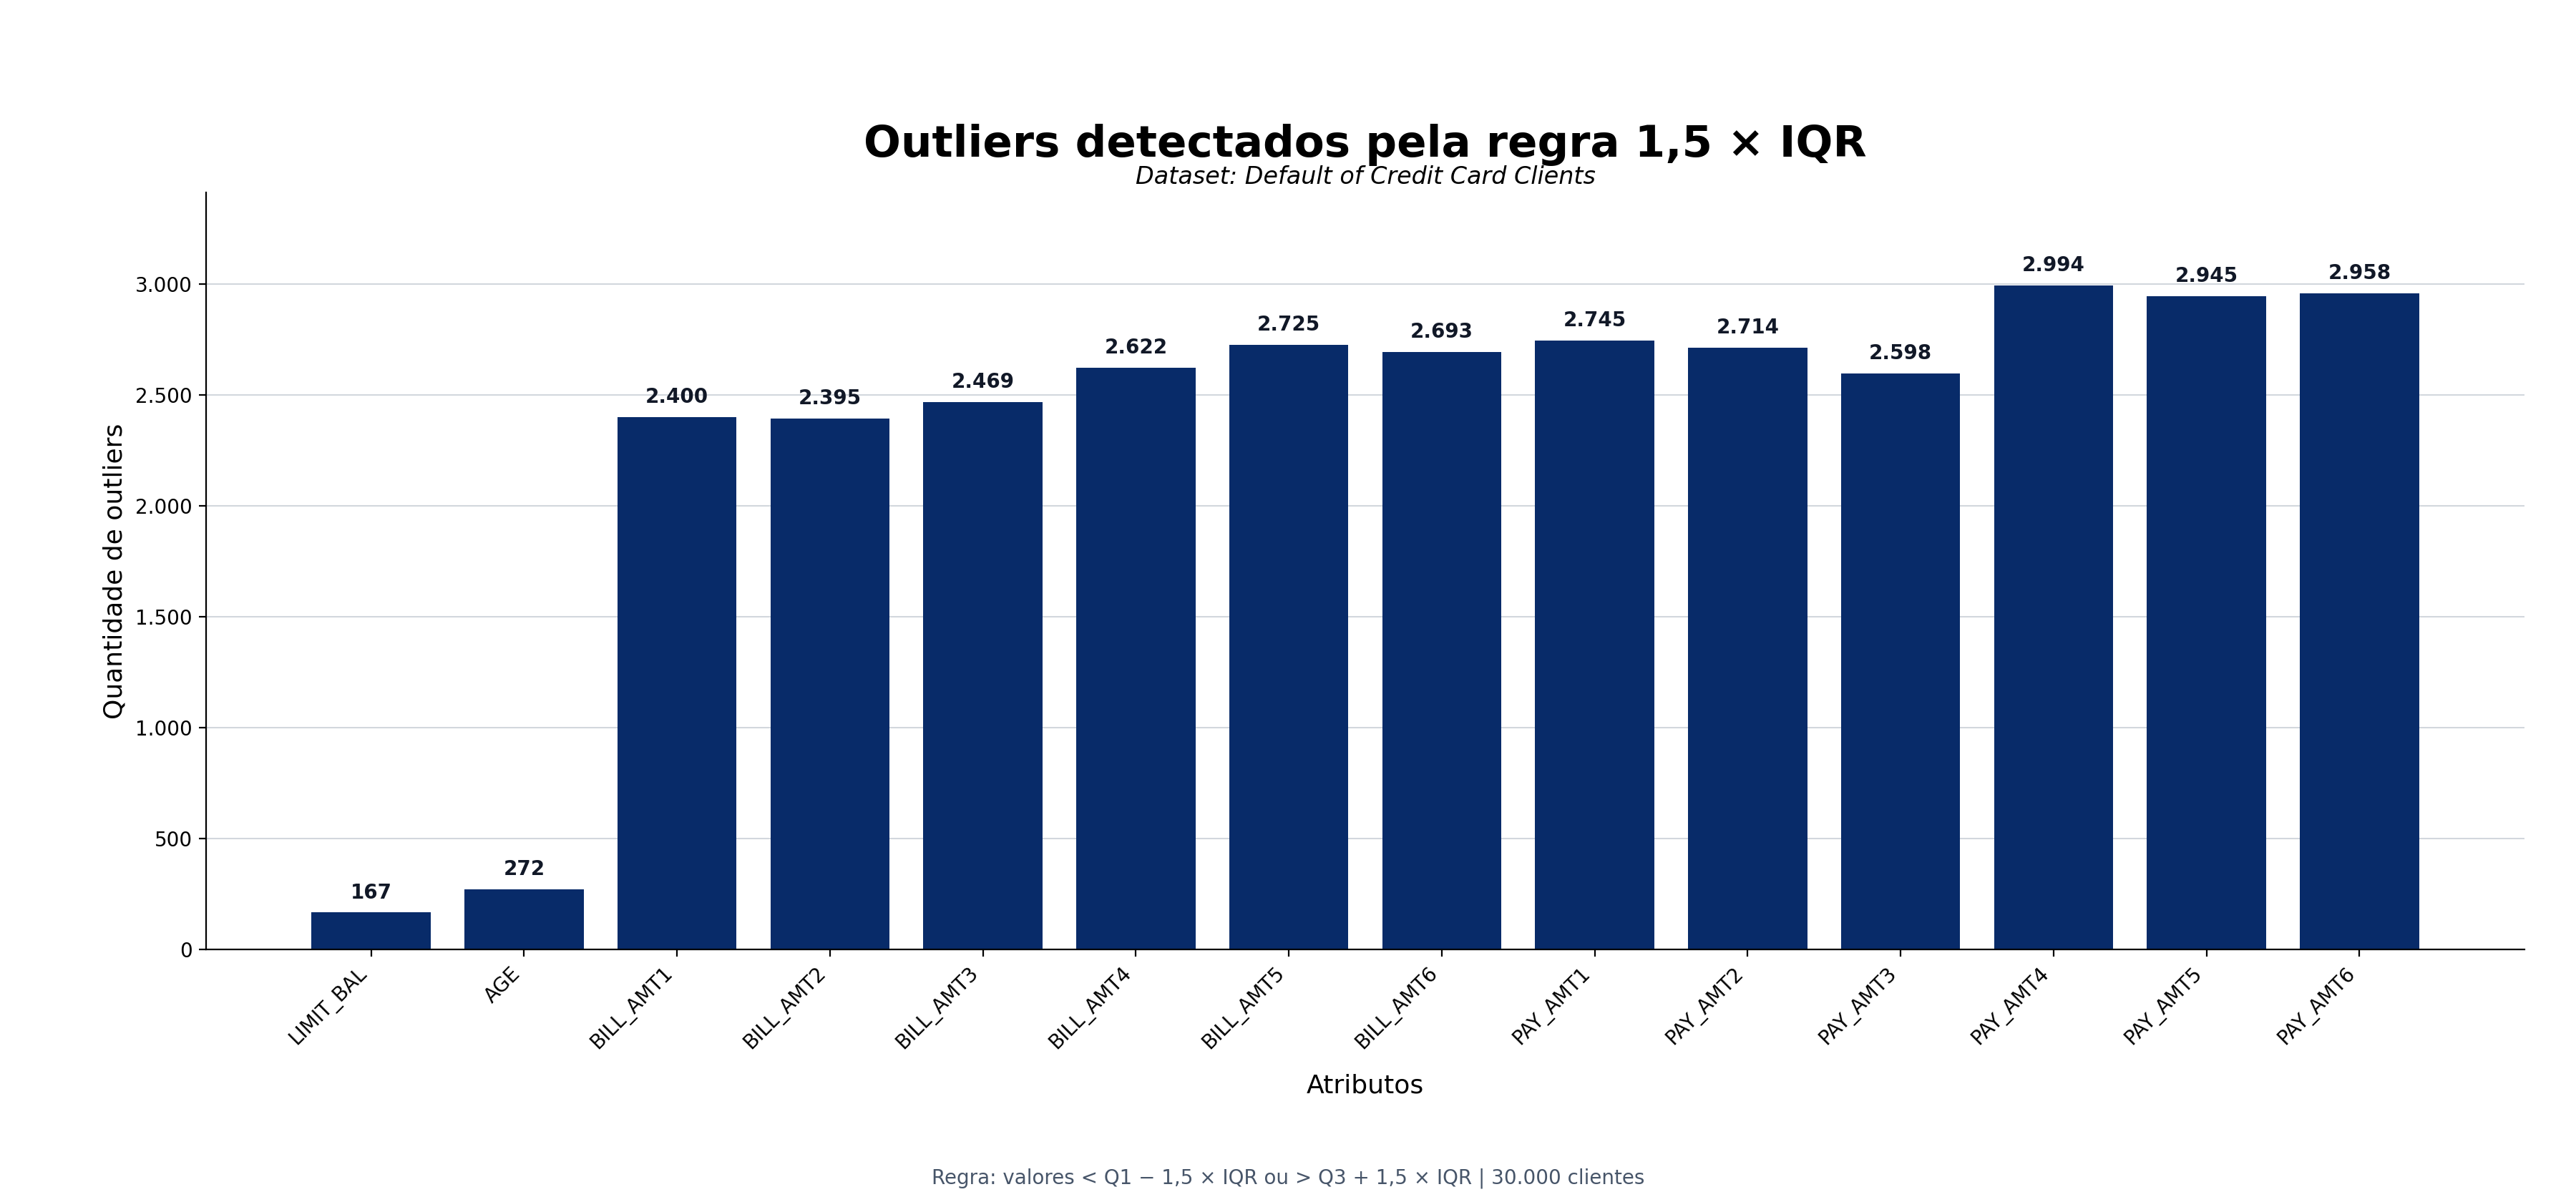
\includegraphics[width=\linewidth]{figures/outliers_iqr.png}\\[-2pt]
{\small\textbf{Figura 3.} Quantidade de valores sinalizados por atributo na base completa.}
\end{center}

\textbf{Faixas observadas}
\begin{center}
\small
\begin{tabularx}{\linewidth}{@{}llXrr@{}}
\toprule
Campo & Atributo & Significado & Mínimo & Máximo\\
\midrule
X1 & \texttt{LIMIT\_BAL} & Limite de crédito (NT\$) & 10.000 & 1.000.000\\
X5 & \texttt{AGE} & Idade (anos) & 21 & 79\\
X12 & \texttt{BILL\_AMT1} & Fatura de setembro (NT\$) & $-165.580$ & 964.511\\
X14 & \texttt{BILL\_AMT3} & Fatura de julho (NT\$) & $-157.264$ & 1.664.089\\
X19 & \texttt{PAY\_AMT2} & Pagamento de agosto (NT\$) & 0 & 1.684.259\\
\bottomrule
\end{tabularx}
\end{center}

O pagamento de agosto teve \textbf{mediana de NT\$ 2.009} e \textbf{média de
NT\$ 5.921,16}. O maior pagamento nesse mês foi de NT\$ 1.684.259.

\newpage
\section{Metodologia}
\subsection*{Como dividimos os dados}
Rodamos os experimentos em Python 3.12 e scikit-learn 1.7.2, com semente
42. Reservamos a primeira de cinco partições estratificadas por grupos
para teste (5.999 registros, 21,67\% da classe 1). O treino recebeu os
24.001 restantes (22,23\% da classe 1). Cada grupo reúne registros com
preditores idênticos, inclusive quando as classes são diferentes.

No treino, usamos as mesmas três dobras estratificadas por grupos para
todos os modelos. Duas servem para ajustar o modelo e uma para validar,
em rodízio. Escolhemos o maior F1 médio de cada modelo (em empate, o
primeiro da grade). Depois, reajustamos no treino completo e avaliamos no teste reservado.

\subsection*{Preparo comum aos quatro modelos}
Retiramos \texttt{ID} dos preditores e usamos \texttt{default payment next
month} como alvo. Aplicamos \textit{one-hot} a \texttt{SEX},
\texttt{EDUCATION}, \texttt{MARRIAGE} e aos seis campos de status de
pagamento (\status{0}, \status{2} a \status{6}). Cada código observado
em cada coluna ganhou um indicador de 0 ou 1, incluindo os códigos
$-2$ e 0 nos campos de pagamento. O codificador ignora categorias que
só aparecem na validação ou no teste.

A base estava completa. A imputação usaria a mediana nos numéricos e a
moda nos categóricos. Ajustamos as transformações no treino de cada
dobra e mantivemos o limiar padrão, a proporção das classes e pesos iguais.

\subsection*{Algoritmos ensinados em aula}

\subsubsection*{1. k-NN}
\textbf{Funcionamento.} Usa a distância euclidiana
$d(x,v)=\sqrt{\sum_j(x_j-v_j)^2}$ para localizar os $k$ vizinhos mais
próximos. Cada vizinho tem um voto. A classe mais votada é a previsão
e a fração de votos da classe 1 é o escore.

\textbf{Justificativa da escolha.} Permite testar se clientes com
históricos financeiros parecidos também têm resultados parecidos.

\textbf{Parâmetros e preparo.} Testamos $k=15$ e $k=45$. O primeiro dá
mais peso à vizinhança imediata. O segundo consulta um grupo maior, o que
reduz o efeito de um cliente isolado. Padronizamos \texttt{AGE},
\texttt{LIMIT\_BAL}, \texttt{BILL\_AMT1} a \texttt{6} e
\texttt{PAY\_AMT1} a \texttt{6}, usando $z=(x-\mu)/\sigma$ com a
média e o desvio-padrão do treino em cada coluna. Assim, a unidade
monetária não domina a distância só por causa da escala.

\subsubsection*{2. Árvore de decisão (CART)}
\textbf{Funcionamento.} A árvore escolhe a regra que mais reduz o Gini
($1-\sum_j p_j^2$, com $p_j$ igual à proporção da classe $j$ no nó).
Para avaliar a regra, pondera o Gini dos dois grupos pelo tamanho de cada
um. O cliente segue as regras até uma folha e recebe a classe mais
frequente ali.

\textbf{Justificativa da escolha.} As regras permitem explicar quais
condições, como um histórico de atraso, levaram a uma classificação.

\textbf{Parâmetros e preparo.} Usamos o critério Gini e testamos
\texttt{max\_depth} de 4 e 8 para comparar uma árvore mais simples com
outra que admite regras mais detalhadas. Mantivemos os valores numéricos
na escala original, pois a árvore compara cada atributo com um limiar.

\newpage
\subsection*{Algoritmos não ensinados em aula}

\subsubsection*{3. Regressão logística}
\textbf{Funcionamento.} Aprende um peso para cada característica dos
clientes. Para um novo cliente, combina as características em uma
pontuação $s=w^\top x+b$ e aplica a função sigmoide:
\[
   p=\frac{1}{1+e^{-s}}.
\]
O resultado $p$ é a probabilidade estimada de inadimplência. O modelo
prevê a classe 1 quando $p>0{,}5$. No treino, a perda logarítmica penaliza
previsões distantes do resultado observado. A penalização L2 acrescenta
um termo proporcional a $\lVert w\rVert_2^2=\sum_j w_j^2$, fazendo
coeficientes grandes custarem mais.

\textbf{Justificativa da escolha.} É uma referência simples para comparar
com as árvores e fornece um escore de risco. Os coeficientes ajudam a
explicar como cada atributo se associa à previsão, mantendo os outros fixos.

\textbf{Parâmetros e preparo.} Comparamos $C=0{,}1$ e $C=1{,}0$.
Quanto menor $C$, mais forte é a penalização L2. Usamos o otimizador
\texttt{lbfgs}, com limite de 500 iterações. As 14 variáveis numéricas
receberam a mesma padronização por z-score do k-NN, o que coloca os
atributos em escalas comparáveis para a penalização.

\textbf{Pseudocódigo}
\begin{enumerate}\setlength{\itemsep}{0pt}
  \item Receber os dados preparados, os rótulos e o valor de $C$. Iniciar os pesos e o intercepto.
  \item Calcular as probabilidades pela sigmoide e a perda com a penalização L2.
  \item Ajustar os pesos e o intercepto com L-BFGS até convergir ou atingir o limite.
  \item Para um novo cliente, calcular $p$ e prever inadimplência se $p>0{,}5$.
\end{enumerate}

\subsubsection*{4. Random Forest}
\textbf{Funcionamento.} Treina várias árvores de decisão, cada uma com
uma amostra de clientes sorteada com reposição. Em cada divisão, a árvore
considera um subconjunto aleatório de atributos e usa Gini para escolher
a regra. Para um novo cliente, cada árvore estima a probabilidade de
inadimplência pela proporção da classe 1 na folha. A floresta tira a
média das probabilidades: $\bar p=(p_1+\cdots+p_{80})/80$. Se
$\bar p>0{,}5$, prevê a classe 1.

\textbf{Justificativa da escolha.} A floresta permite captar relações não
lineares e combinações de atributos, como valores de fatura e atrasos.
A média das árvores reduz a dependência das regras de uma única árvore.

\textbf{Parâmetros e preparo.} Fixamos \texttt{n\_estimators=80} e
\texttt{bootstrap=True}. O sorteio de atributos usa \texttt{sqrt},
a raiz quadrada do total, para diversificar as árvores. Testamos
\texttt{max\_depth} de 8 e 14 para comparar dois níveis de
complexidade. Mantivemos a escala original das variáveis numéricas.

\textbf{Pseudocódigo}
\begin{enumerate}\setlength{\itemsep}{0pt}
  \item Para cada uma das 80 árvores, sortear uma amostra do treino com reposição.
  \item Em cada nó, sortear atributos candidatos e escolher uma divisão por Gini.
  \item Parar no limite de profundidade ou quando não houver divisão válida.
  \item Para um novo cliente, tirar a média das probabilidades das árvores e prever a classe.
\end{enumerate}

\newpage

\subsection*{Medidas de avaliação}
VP, VN, FP e FN são verdadeiros positivos, verdadeiros negativos, falsos
positivos e falsos negativos, respectivamente. A classe positiva é a 1.
\begin{align*}
 F_1\ (\text{classe 1}) &= \frac{2\,\mathrm{VP}}{2\,\mathrm{VP}+\mathrm{FP}+\mathrm{FN}} \\
 \text{Acurácia balanceada} &= \frac{1}{2}\left(
  \frac{\mathrm{VP}}{\mathrm{VP}+\mathrm{FN}} +
  \frac{\mathrm{VN}}{\mathrm{VN}+\mathrm{FP}}\right) \\
 \text{ROC-AUC} &= P(s_{+}>s_{-}) + \tfrac{1}{2}P(s_{+}=s_{-}) \\
 \text{Acurácia} &= \frac{\mathrm{VP}+\mathrm{VN}}{\mathrm{VP}+\mathrm{VN}+\mathrm{FP}+\mathrm{FN}}.
\end{align*}
$F_1$ combina precisão e sensibilidade da classe 1 (é zero se o denominador
for zero). Acurácia balanceada dá o mesmo peso à sensibilidade e à
especificidade. ROC-AUC mede a ordenação dos escores $s_{+},s_{-}$ de casos
positivo e negativo, sem fixar limiar, e usa a probabilidade prevista da
classe 1. Acurácia é uma referência; seu valor isolado pode esconder erros
da classe minoritária. As demais métricas e as matrizes usam a classe
prevista pelo estimador.

\section{Resultados e discussão}
\textbf{Tabela 1.} Validação cruzada no treino: média $\pm$ desvio-padrão
nas três dobras. Asterisco: configuração selecionada por F1 da classe 1
na respectiva família. \emph{Prof.} é a profundidade máxima.

\begingroup\small\setlength{\tabcolsep}{3.5pt}
\begin{tabular*}{\linewidth}{@{\extracolsep{\fill}}llrrrr@{}}
\toprule
Modelo & Config. & F1 classe 1 & ROC-AUC & Ac. balanceada & Acurácia\\
\midrule
\linhasValidacao
\bottomrule
\end{tabular*}
\endgroup

\vspace{9pt}
\textbf{Tabela 2.} Resultados no mesmo teste reservado para os quatro
modelos reajustados no treino inteiro.

\begingroup\small\setlength{\tabcolsep}{3.5pt}
\begin{tabular*}{\linewidth}{@{\extracolsep{\fill}}llrrrr@{}}
\toprule
Modelo & Config. & F1 classe 1 & ROC-AUC & Ac. balanceada & Acurácia\\
\midrule
\linhasTeste
\bottomrule
\end{tabular*}
\endgroup

\newpage
\subsection*{Matrizes de confusão}
\begin{center}
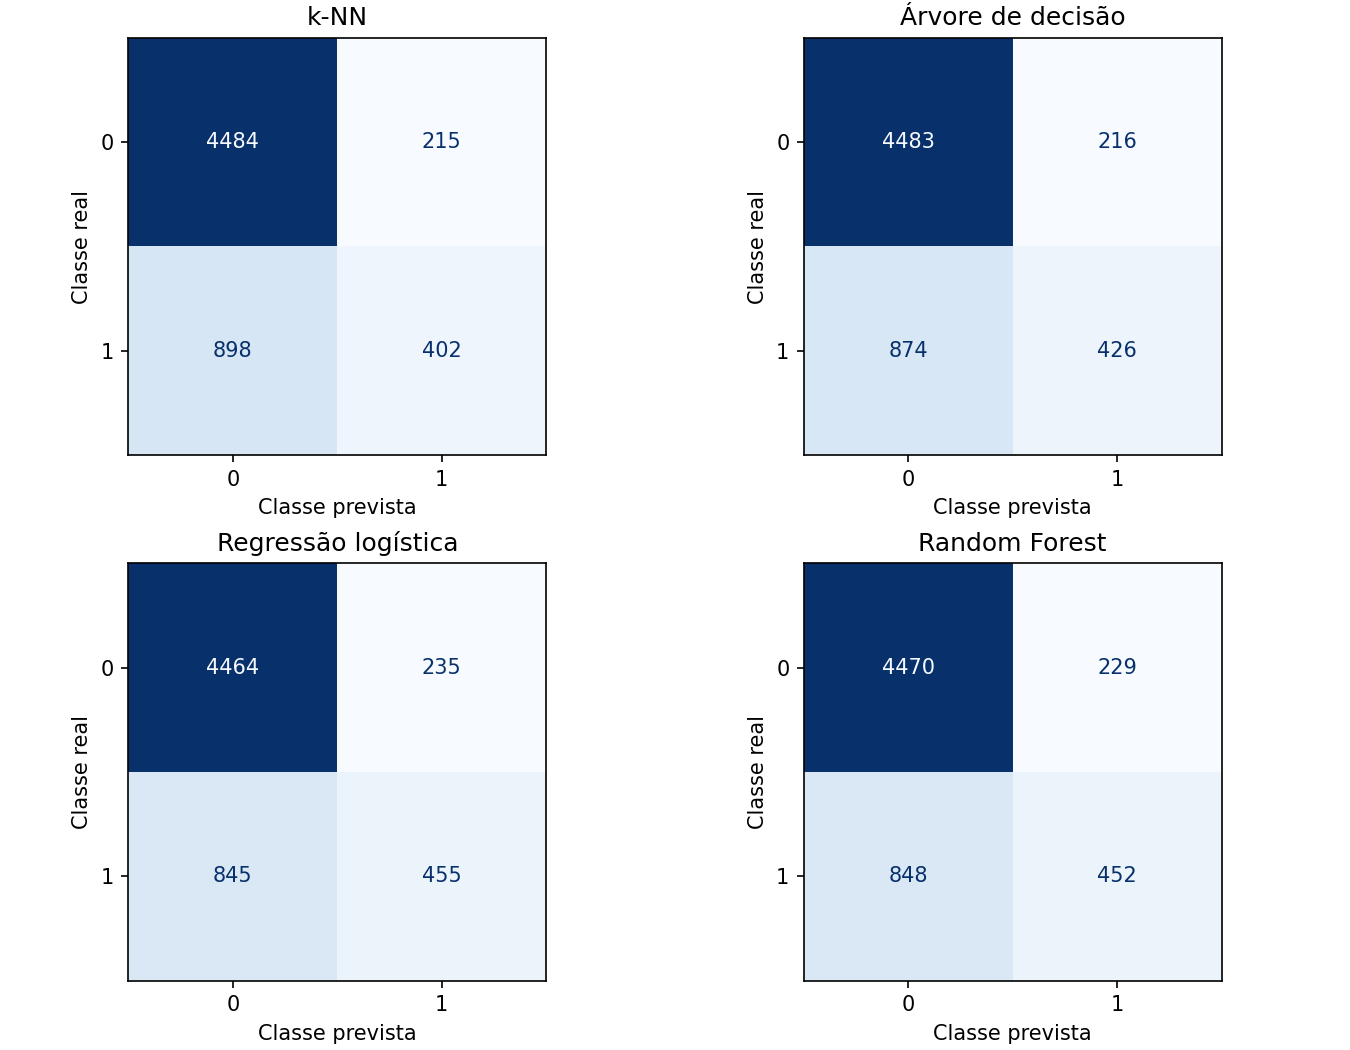
\includegraphics[width=.77\linewidth]{figures/matrizes_confusao.png}\\[-2pt]
{\small\textbf{Figura 4.} Teste reservado. As linhas mostram as classes reais e
as colunas mostram as previstas. A classe 1 indica inadimplência.}
\end{center}

\subsection*{Discussão}
A regressão logística teve o maior F1 no teste (0,4573) e ficou muito
próxima da Random Forest (0,4563). As duas também tiveram acurácia
balanceada perto de 0,65. A floresta teve a maior ROC-AUC, 0,7825 contra
0,7720 da regressão. Isso indica que a floresta ordenou melhor os
clientes pelo risco. No limiar padrão de 0,5, as duas tiveram resultados
próximos. O k-NN e a árvore ficaram atrás nessas três métricas.

\textbf{Efeito dos parâmetros.}
Ao passar de 15 para 45 vizinhos, o F1 médio do k-NN caiu de 0,410 para
0,371, enquanto a ROC-AUC subiu de 0,728 para 0,746. Com 45 vizinhos,
são necessários 23 votos para prever inadimplência. A classe 1 é bem
menos frequente na base, o que pode dificultar que ela alcance essa
maioria. A proporção de votos também passa a ter mais valores possíveis,
o que pode ajudar a ordenar os clientes. Essas são hipóteses. A sensibilidade
por configuração não foi registrada na validação.

Na Random Forest, a profundidade 14 elevou o F1 de 0,441 para 0,462.
A ROC-AUC ficou perto de 0,776 nas duas configurações. Na árvore de
decisão, a profundidade 8 teve F1 maior (0,458 contra 0,450).
A árvore de profundidade 4 teve ROC-AUC e acurácia ligeiramente maiores.
Na regressão, mudar $C$ de 0,1 para 1 teve pouco efeito nos valores testados
(F1 de 0,469 e 0,470).

\newpage
\textbf{Erros e classes desbalanceadas.}
Todos os modelos deixaram passar cerca de dois terços dos inadimplentes.
A regressão teve o menor número de falsos negativos, 845 de 1.300.
Dos 690 clientes sinalizados pela regressão, 455 ficaram inadimplentes,
o que dá cerca de 66\% de precisão. Se deixar passar um inadimplente
custar mais do que sinalizar um cliente que paga em dia, essa baixa
sensibilidade é importante para a decisão.

Prever sempre a classe 0 já daria 78,33\% de acurácia no teste (4.699 de
5.999) e deixaria passar todos os inadimplentes. Os modelos ganharam
de 3,12 a 3,72 pontos percentuais de acurácia sobre essa referência.
Por isso, também avaliamos o F1 da classe 1, a ROC-AUC e a acurácia
balanceada. Esta última ficou perto de 0,65 para a regressão e a
floresta, enquanto a referência que sempre prevê a classe 0 teria 0,50.

\textbf{O que pode ter influenciado os resultados.}
O atraso mais recente (\status{0}) pode ajudar a explicar por que a
regressão ficou próxima da floresta. É uma hipótese, pois o experimento
não mediu a importância dos atributos. Com \textit{one-hot}, a regressão
aprende um peso para cada indicador de status. No k-NN, os indicadores
de seis meses e os 12 valores de fatura e pagamento entram no mesmo
cálculo de distância. A correlação entre as faturas e o número de
indicadores podem diluir o peso dos atributos mais relevantes. Além
disso, 21 grupos têm preditores idênticos e classes diferentes, o que
dificulta separar todos os casos usando apenas esses atributos.

\subsection*{Recomendação do grupo}
Recomendamos a regressão logística com $C=1$. Ela teve o maior F1 da
classe 1 e a maior acurácia balanceada no teste. Seus coeficientes
também facilitam a explicação: mantendo os demais atributos fixos, cada
coeficiente indica como seu atributo se associa ao logaritmo das chances
de inadimplência. O indicador de dois meses de atraso em setembro, por
exemplo, tem um coeficiente próprio. O experimento não analisou o
sinal nem o tamanho desse coeficiente. O tempo de treinamento também
não foi medido.

Se o objetivo fosse ordenar clientes por risco, a Random Forest seria
uma alternativa pela ROC-AUC maior em 0,0106. Para uma decisão
individual, consideramos pequeno esse ganho diante da dificuldade
de explicar o resultado de 80 árvores. Mesmo para a regressão, o
limiar padrão de 0,5 deixou passar 65\% dos inadimplentes. Um limiar de
uso prático precisaria ser validado considerando o custo dos dois
tipos de erro.

\newpage
\section{Conclusões}
A regressão logística e a Random Forest ficaram próximas no F1 e na
acurácia balanceada. A floresta ordenou melhor os escores de risco
pela ROC-AUC. No k-NN, aumentar $k$ melhorou a ROC-AUC e reduziu o F1
na validação. Esses resultados mostram por que escolhemos a métrica de
acordo com o tipo de erro que mais importa.

A maior limitação foi a baixa detecção da classe 1. No limiar padrão,
sem pesos de classe nem reamostragem, a sensibilidade ficou entre
30,9\% e 35,0\%. Testamos apenas dois valores por modelo e usamos uma
única partição de teste. Também mantivemos códigos sem significado
documentado e não incorporamos custos reais de decisão.

Como próximos passos, compararíamos limiares na validação e testaríamos
pesos de classe nos modelos compatíveis. Também avaliaríamos atributos
derivados, como pior atraso, proporção do limite usado e proporção da
fatura paga. Outras extensões seriam testar \textit{gradient boosting},
verificar a calibração das probabilidades e avaliar diferenças de
desempenho entre grupos quando sexo e estado civil são usados.

\section{Referências}
\begingroup\small
\begin{enumerate}
  \item YEH, I.-C. \textit{Default of Credit Card Clients}. UCI Machine
  Learning Repository, 2009.\\
  DOI: \href{https://doi.org/10.24432/C55S3H}{10.24432/C55S3H}.
  Licença \href{https://creativecommons.org/licenses/by/4.0/}{CC BY 4.0}.
  \item YEH, I.-C.; LIEN, C.-H. The comparisons of data mining techniques for the predictive
  accuracy of probability of default of credit card clients. \textit{Expert Systems with
  Applications}, v.~36, n.~2, p.~2473--2480, 2009.
  DOI: \href{https://doi.org/10.1016/j.eswa.2007.12.020}{10.1016/j.eswa.2007.12.020}.
  \item \href{https://scikit-learn.org/1.7/}{scikit-learn 1.7}: classificadores, pré-processamento,
  métricas e validação. \href{https://pandas.pydata.org/docs/}{pandas 2.3.3} e
  \href{https://xlrd.readthedocs.io/}{xlrd 2.0.2}: leitura e tabulação.
  \href{https://matplotlib.org/stable/}{Matplotlib 3.10.8}: figuras.
  \item FARIA, E. R. \textit{Trabalho Final: Classificação} e materiais de
  aula 5 (k-NN), 7 (árvores de decisão) e 9 (avaliação de classificação).
  Mineração de Dados, Universidade Federal de Uberlândia, 2026.
  \item OPENAI. ChatGPT. \href{https://chatgpt.com/share/6b04da96-4530-83e9-98f6-85088f31c754}{Explicação geral e geração de gráficos.}
  \item OPENAI. ChatGPT. \href{https://chatgpt.com/share/6b04daa8-973c-83e9-92fe-b00af9c01be8}{Discussão sobre a escolha dos algoritmos do trabalho.}
  \item Repositório do trabalho no GitHub. \url{https://github.com/LuksbellN/Trabalho-MD-Final}
\end{enumerate}
\endgroup

\newpage
\section*{Uso de IA generativa}
\textbf{Ferramentas.} Usamos Devin (Cognition AI) para apoiar a análise
exploratória, os experimentos em Python, a geração de gráficos e a redação
preliminar. Usamos ChatGPT (OpenAI) para esclarecer dúvidas sobre
pré-processamento, algoritmos e métricas e para revisar o relatório.

\textbf{Chats utilizados}
\begin{itemize}\setlength{\itemsep}{1pt}
  \item Explicação geral e geração de gráficos.\\
  \url{https://chatgpt.com/share/6b04da96-4530-83e9-98f6-85088f31c754}
  \item Discussão sobre a escolha dos algoritmos do trabalho.\\
  \url{https://chatgpt.com/share/6b04daa8-973c-83e9-92fe-b00af9c01be8}
\end{itemize}

\textbf{Verificação.} Todos os integrantes do grupo revisaram a discussão
e a recomendação e conferiu a reprodução dos notebooks e das tabelas.
Nesta revisão, conferimos as configurações no notebook e nos CSVs,
recalculamos o IQR, as contagens de classe e as estatísticas destacadas
no texto e revisamos as fórmulas e os pseudocódigos.

\subsection*{Prompts utilizados com o Devin (Cognition AI)}
Os exemplos de parâmetros abaixo fazem parte dos pedidos. As
configurações executadas estão na metodologia e nas tabelas de resultados.

\begin{enumerate}
  \item ``Faça a análise exploratória do dataset, instâncias e atributos, tipos e significados, atributo classe e distribuição, desbalanceamento, valores ausentes, duplicatas, inconsistências e códigos não documentados, gere um relatório geral de seus achados''.
  \item ``Monte um protocolo de execução dos algoritmos, com validação cruzada estratificada por grupos em 3 dobras de registros de treinos. Desenvolva, rode e compare os algoritmos de KNN, arvore de decisão, Regressão logística e Random Forest com 2 configurações cada (exemplo: KNN -> k=5 e k=21, Arvore de decisão -> max\_depth = 4 e max\_depth=8, Regressão Logística -> C = 0.1 e C=1 e Random forest -> max\_depth = 1 e max\_depth = 10). Use métricas adequadas ao desbalanceamento, apresente as fórmulas e salve os CSVs e as matrizes de confusão.''
  \item ``Valide os algoritmos utilizados se condizem com o meu entendimentos do Random forest e da Regressão Logística. Procure por data leakage e possíveis ajustes de hiperparâmetros no conjunto de teste para cada uma das 3 dobras.''
\end{enumerate}

\end{document}
